% This is the Reed College LaTeX thesis template. Most of the work 
% for the document class was done by Sam Noble (SN), as well as this
% template. Later comments etc. by Ben Salzberg (BTS). Additional
% restructuring and APA support by Jess Youngberg (JY).
% Your comments and suggestions are more than welcome; please email
% them to cus@reed.edu
%
% See http://web.reed.edu/cis/help/latex.html for help. There are a 
% great bunch of help pages there, with notes on
% getting started, bibtex, etc. Go there and read it if you're not
% already familiar with LaTeX.
%
% Any line that starts with a percent symbol is a comment. 
% They won't show up in the document, and are useful for notes 
% to yourself and explaining commands. 
% Commenting also removes a line from the document; 
% very handy for troubleshooting problems. -BTS

% As far as I know, this follows the requirements laid out in 
% the 2002-2003 Senior Handbook. Ask a librarian to check the 
% document before binding. -SN

%%
%% Preamble
%%
% \documentclass{<something>} must begin each LaTeX document
\documentclass[12pt,twoside]{reedthesis}
% Packages are extensions to the basic LaTeX functions. Whatever you
% want to typeset, there is probably a package out there for it.
% Chemistry (chemtex), screenplays, you name it.
% Check out CTAN to see: http://www.ctan.org/
%%
\usepackage{graphicx,latexsym} 
\usepackage{amssymb,amsthm,amsmath}
\usepackage{longtable,booktabs,setspace} 
\usepackage{chemarr} %% Useful for one reaction arrow, useless if you're not a chem major
\usepackage[hyphens]{url}
\usepackage{rotating}
\usepackage{natbib}
\usepackage{hhline}
\usepackage{multirow}
\usepackage{adjustbox}
\usepackage{algorithm,algpseudocode}
\usepackage{changepage}

%%% begin alex commands %%%
\usepackage{hyperref}
\hypersetup{
    colorlinks=true,
    linkcolor=blue,
    filecolor=magenta,      
    urlcolor=cyan,
}
\newcommand{\Gates}{\text{Gates}}
\newcommand{\InputWires}{\text{InputWires}}
\newcommand{\OutputWires}{\text{OutputWires}}
\newcommand{\Wires}{\text{Wires}}
\newcommand{\Enc}{\operatorname{Enc}}
\newcommand{\Dec}{\operatorname{Dec}}
\newcommand{\EncInv}{\Enc^{-1}}
\newcommand{\EncDKC}{\operatorname{EncDKC}}
\newcommand{\DecDKC}{\operatorname{DecDKC}}
\newcommand{\EncDKCInv}{\EncDKC^{-1}}
\newcommand{\compIndist}{\approx_D}
\newcommand{\outputrv}{{\sf output}}
\newcommand{\viewrv}{{\sf view}}

\newcounter{defcounter}
\setcounter{defcounter}{0}
\newenvironment{definition}{\medskip\noindent\refstepcounter{defcounter}{\bf Definition \thedefcounter}\hspace*{2pt}}{\hspace*{\fill}\nopagebreak[4]$\diamondsuit$\medskip}  

\newenvironment{blockquote}{%
  \par%
  \medskip
  \leftskip=4em\rightskip=2em%
  \noindent\ignorespaces}{%
  \par\medskip}

%%% end alex commands %%%



% Comment out the natbib line above and uncomment the following two lines to use the new 
% biblatex-chicago style, for Chicago A. Also make some changes at the end where the 
% bibliography is included. 
%\usepackage{biblatex-chicago}
%\bibliography{thesis}

% \usepackage{times} % other fonts are available like times, bookman, charter, palatino

\title{Two Party Computation}
\author{Alex Ledger}
% The month and year that you submit your FINAL draft TO THE LIBRARY (May or December)
\date{May 2015}
\division{Mathematics and Natural Sciences}
\advisor{Adam Groce}
%If you have two advisors for some reason, you can use the following
%\altadvisor{Your Other Advisor}
%%% Remember to use the correct department!
\department{Mathematics}
% if you're writing a thesis in an interdisciplinary major,
% uncomment the line below and change the text as appropriate.
% check the Senior Handbook if unsure.
%\thedivisionof{The Established Interdisciplinary Committee for}
% if you want the approval page to say "Approved for the Committee",
% uncomment the next line
%\approvedforthe{Committee}

\setlength{\parskip}{0pt}
%%
%% End Preamble
%%
%% The fun begins:
\begin{document}

  \maketitle
  \frontmatter % this stuff will be roman-numbered
  \pagestyle{empty} % this removes page numbers from the frontmatter

% Acknowledgements (Acceptable American spelling) are optional
% So are Acknowledgments (proper English spelling)
    \chapter*{Acknowledgements}
	I want to thank a few people.

% The preface is optional
% To remove it, comment it out or delete it.
\chapter*{Preface}
This is an example of a thesis setup to use the reed thesis document class.



\chapter*{List of Abbreviations}
	You can always change the way your abbreviations are formatted. Play around with it yourself, use tables, or come to CUS if you'd like to change the way it looks. You can also completely remove this chapter if you have no need for a list of abbreviations. Here is an example of what this could look like:

\begin{table}[h]
\centering % You could remove this to move table to the left
\begin{tabular}{ll}
	\textbf{ABC}  	&  American Broadcasting Company \\
	\textbf{CBS}  	&  Columbia Broadcasting System\\
	\textbf{CDC}  	&  Center for Disease Control \\
	\textbf{CIA}  	&  Central Intelligence Agency\\
	\textbf{CLBR} 	&  Center for Life Beyond Reed\\
	\textbf{CUS}  	&  Computer User Services\\
	\textbf{FBI}  	&  Federal Bureau of Investigation\\
	\textbf{NBC}  	&  National Broadcasting Corporation\\
\end{tabular}
\end{table}
	

    \tableofcontents
% if you want a list of tables, optional
    \listoftables
% if you want a list of figures, also optional
    \listoffigures

% The abstract is not required if you're writing a creative thesis (but aren't they all?)
% If your abstract is longer than a page, there may be a formatting issue.
    \chapter*{Abstract}
	The preface pretty much says it all.
	
	\chapter*{Dedication}
	You can have a dedication here if you wish.

  \mainmatter % here the regular arabic numbering starts
  \pagestyle{fancyplain} % turns page numbering back on

%The \introduction command is provided as a convenience.
%if you want special chapter formatting, you'll probably want to avoid using it altogether

\chapter*{Introduction}
     \addcontentsline{toc}{chapter}{Introduction}
\chaptermark{Introduction}
\markboth{Introduction}{Introduction}
% \onehalfspacing
\doublespacing

 Introduction goes here

\chapter{Background}

Multiparty computation (MPC) is the study and creation of protocols for computing a function between multiple parties, such that no party learns the input of any other party.

The idea is best communicated through an example: suppose Alice and Bob are millionaires and wish to determine who is wealthier, but Alice and Bob are also secretive, and do not want to disclose their exact amount of wealth. 
Is there some method by which they can determine who has more money?

The goal of MPC is to design a protocol which will help Alice and Bob solve their problem.
The desired properties of a secure MPC scheme can be informally described as follows:
\begin{itemize}
    \item \textbf{Privacy:} Each party's input is kept secret.
    \item \textbf{Correctness:} The correct answer to the computation is computed.
\end{itemize}

Originally, the goal was to come up with a protocol that was secure and prove that the protocol was secure. 
In more recent times, the focus has shifted to making the MPC faster, fast enough that it can be used regularly in the real world.

If MPC can be made fast enough, it could serve a wide range of applications.
For example, imagine that two companies who operate in a similar industry want to work together, but they don't want to disclose any company research which the other doesn't know.
These companies could a run set intersection function (a function that given two inputs finds their intersection, or overlap), to determine what information they can disclose without giving away important information.

Another interesting example of MPC is to improve the outsourcing of computation.
As it is right now, cloud computing companies, such as Amazon and Google, have really nice computers which they will rent out to you. 
You can pay them someone money, write a program, and run it on their computers. 
The problem is that you may not trust the cloud computing company, and you want some guarantees that they are going to respect the privacy of your computation.
An MPC protocol, in this setting, would allow you to run computation in the cloud, with the guarantee that the inputs to your computation are disguised.

Since the research into MPC has focused on creating a method by which an arbitrary function can be computed securely, the application of MPC beyond what we can presently conceive of. 
It's not unlikely that MPC protocols will become a standard in the internet, where when you access the internet, behind the scenes your access is being is plugged into an MPC protocol, sent off to another computer to do some processing. 
As cryptography improves, research in MPC and other areas of cryptography, the hope is that the security of our computer systems will improve as well.
However, there is no guarantee. 
The modern cryptography needs to implemented and used, perhaps in some cases built into low-level standards, and used correctly.
At this point, the outlook of cryptography is bright, but the future will only be realized positvely if it is actively worked towards.

\section{Tools for MPC}
MPC is a complex construction with many moving parts. 
Each moving part is itself a unique cryptographic primitive, which when combined give rise to MPC.
The following sections give a summary of the crytographic tools required for MPC.

\subsection{Encryption}
Encryption is the process of encoding a message such that only parties with the key can read the message.
As we discuss MPC, we will be using symmetric-key encryption, the case of encryption where encryption and decryption use the same key.
Public key encryption, in constrast, uses two different keys: one key for encryption and a different key for decryption.
While early MPC schemes used public key encryption, modern methods do not require public key encryption, and symmetric-key encryption algorithms are faster, making them preferable.

A symmetric-key encryption protocol is composed of two parts.
The first part is the encryption algorithm which disguises the message, and the second part is the decryption algorithm which unobfuscates the disguised message.
We notate the decryption algorithm, $\Dec$ as $\EncInv$.
We notate encryption and decryption with
\begin{equation}
    \label{eqn:encryption}
    \begin{split}
        \Enc_k (pt) & = ct  \\
        \EncInv_k(ct) & = pt
    \end{split}
\end{equation}
where $pt$ stands for plaintext and is the original message, $ct$ stands for ciphertext and is the encrypted message, and $k$ is the secret key, that only authorized readers of the message hold.
For the algorithm to be effective, the secret key $k$ must be a randomstring of $0$s and $1$s of length $\lambda$.
\footnote{The notion of randomness in cyptoraphy has a precise definition, and in cases where $\lambda$ is large, it is sufficient for $k$ to be pseuodorandom. Pseudorandom also has precise cryptographyic definition.}

$\lambda$ is the security parameter of our protocol.
If we increase $\lambda$, thereby increasing the size of the key, then the encyrption algorithm becomes harder for an adversary to break.

It is useful for MPC to define a specific type of symmetric-key encryption algorithm called a Dual-Key Cipher (DKC) \cite{bellare2012foundations}.
A DKC requires two secret keys to encrypt and decrypt the message, in constrast to classic encryption which only requires one.
It is easy to instantiate a DKC if one has a secure encryption scheme: let $k_0$ and $k_1$ be the two secret keys, and instantiate the DKC as follows:
\begin{equation}
    \begin{split}
        \EncDKC_{k_0, k_1}(pt) = \Enc_{k_1} ( \Enc_{k_0} ( pt )) \\
        \EncDKCInv_{k_0, k_1}(ct) = \EncInv_{k_0} ( \EncInv_{k_1} ( ct )) 
    \end{split}
\end{equation}
This construction of a DKC is slow, and there are many faster methods for instantiating DKCS.
For more information, see \cite{bellare2012foundations}.

\subsection{Boolean Circuit} 
A function for an MPC protocol is represented by a boolean circuit.
A boolean circuit takes as input a sequence of $n$ $0$s and $1$s, (i.e. a value in $\{0,1\}^n$), performs a series of small opreations on the inputs, and outputs a sequence of m $0$s and $1$s (i.e. a value in $\{0,1\}$).
You may have encountered circuits and logical operators in another context, where the inputs and outputs were True and False.
For our usage, True will correspond to the value $1$, and False will corresond to the value $0$. 

The small operations done inside of a circuit are performed by an object called a \emph{gate}.
A gate is composed of three wires: two input wires and one output wire, where a \emph{wire} can have a value either $0$ or $1$.
A gate performs a simpler operation on the two inputs, resulting in a single output bit.
Table \ref{tab:xor} gives the mapping of an XOR gate.

\begin{table}[h]
\label{tab:xor}
\centering
\begin{tabular}{ | l | c || r |}
\hline
x & y & xor(x,y) \\ \hline
1 & 1 & 0 \\ \hline
1 & 0 & 1 \\ \hline
0 & 1 & 1 \\ \hline
0 & 0 & 0 \\ \hline
\end{tabular}
\caption{The mapping of an XOR gate.}
\end{table}

A circuit is a combination of gates. 
In fact, a circuit built out of only AND gates, XOR gates and NOT gates can compute any function or algorithm.
\textbf{Find details and citation} In other words, if there's some algorithm that do it, then there is some circuit that can do it as well.
Figure \ref{fig:less_than_circuit} shows the circuit representation of the less than function, $f$ as specified in equation \ref{eqn:less_than}.

\begin{figure}[h]
    \centering
    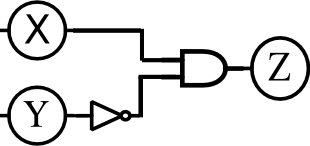
\includegraphics[scale=0.75]{images/drawing.png}
    \label{fig:less_than_circuit}
    \caption{A circuit that computes the less or equal to function, equivalent to $f$ for input of two one-bit values. \textbf{TODO, add truth table?}}
\end{figure}

\subsection{Technical Definition of a Circuit}
It is useful at times to have a formal definition of a circuit.
Here we give a formal definition of a circuit proposed by BHR in \cite{bellare2012foundations}.

A circuit is formalized by a 6-tuple $g = (n,m,q,A,B,G)$, where $n$ is the number of inputs, $m$ is the number of outputs and $q$ is the number of gates.
We define $r = n + q$ to the number of wires inside of the circuit.
We let $\Wires = \{1,\ldots, n+q\}, \InputWires = \{1,\ldots, n\}, \OutputWires = \{n+1-m+1, \ldots,n+q\}$, and $\Gates = \{n+1, \ldots, n+q\}$.
Then $A : \Gates \to \Wires \setminus \OutputWires$ identifies each gate's first incoming wire.
And $B : \Gates \to \Wires \setminus \OutputWires$ identifies each gate's second incoming wire.
Finally, $G: \Gates \times \{0,1\}^2 \to \{0,1\}$ identifies the functionality of each gate.

% TODO - if we want - 
% For example, the less than circuit shown in figure \ref{fig:less_than_circuit} has values:

\newcommand{\Gb}{\operatorname{Gb}}
\newcommand{\En}{\operatorname{En}}
\newcommand{\De}{\operatorname{De}}
\newcommand{\Ev}{\operatorname{Ev}}
\newcommand{\ev}{\operatorname{ev}}
\newcommand{\evcirc}{\ev_{circ}}

\newcommand{\fbar}{f^-}
\newcommand{\Topo}{\operatorname{Topo}}
\renewcommand{\algorithmicrequire}{\textbf{Input:}}
\renewcommand{\algorithmicensure}{\textbf{Output:}}

To evaluate a circuit, we use a canonical algorithm $\evcirc$, which takes as input a function $f$ (encoded as a string) and a string $x = x_1 x_2 \ldots x_n$ and does the following:

\begin{algorithm}
\caption{$\evcirc$}
\label{alg:evcirc}
\begin{algorithmic}
\Require Function $f$ and String $x = x_1, \ldots x_n$.
\Ensure Output of function $f$ on input $x$.
\State $(n,m,a,A,B,G) \gets f$
\Comment parse $f$ as a circuit
\For{$g = n+1$ to $n+q$} 
\Comment loop over all gates.
\State $a \gets A(g)$
\Comment compute each gate
\State $b \gets B(g)$
\State $x_g \gets G_g(x_a, x_b)$
\EndFor \\
\Return $x_{n+q-m+1} \ldots x_{n+q}$
\end{algorithmic}
\end{algorithm}

\subsection{Computational Indistinguishability and the DDH Assumption} 
\label{sctn:DDH}
\textbf{Add in computational indist defn here. use lindellpinkas paper}
\textbf{Check if this is ever used - it is used. see eqn 1.6, ensebles}
\textbf{Give encryptiong example?}

When a cryptographic scheme is said to be \textit{secure}, cryptographers actually mean something much more precise. 
It means that an adversary can beat the scheme only if the adversary can tackle the hardness assumptions on which the scheme is based.
Hardness assumption, in the way I'm using it, means a problem, like factoring a number or finding the greatest common divisor of two numbers.
At a high level then a cryptographic scheme is secure so long as there is no efficient algorithm for solving the underlying problem.

For example, say we have some encryption scheme with has algorithms $\Enc$ and $\EncInv$.
Then in order to make the statement ``$\Enc$ is secure'' substantial and precise, we might say that ``an adversary can determine $m$ given $\Enc_k(m)$ and the $\Enc$ algorithm if and only if the same adversary can solve problem $P$''.
The real trick for making a good encryption algorithm is threefold: (1) finding a problem $P$ which is hard to solve, (2) making $\Enc$ dependent on $P$, and (3) ensuring that $\Enc^{-1}$ is efficient to solve (because we need to be able to decrypt our messages quickly).

This formulation of security turns out to be useful for a number of reasons. 
One reason is that we will know when the scheme becomes insecure. 
If the underlying problem, like factoring large numbers, becomes solvable efficiently, then we immediately know that our scheme in insecure.
There is a major disadvantage to this formulationation.
Once researchers found a few good hardness assumption, almost all cryptographic schemes became dependent on these problems; all of the eggs were put in a few baskets. 
So if one big problem is found to have an efficient solution, such as factoring prime numbers, then many cryptographic schemes will break.

A common hardness assumption is the Decisional Diffie-Helman Assumption (DDH Assumption), an assumption about solving a problem concerning discrete logs.

Informally, the DDH assumption is:
\begin{equation}
	\label{eqn:DDH}
	\begin{split}
	& \qquad \text{Let $G$ be a group of order $q$ with generator $g$.} \\
	& \qquad \text{Let $a, b$ and $c$ be random elements from $\mathbb{Z}_q$.} \\
	& \qquad \text{Then, $(g^a, g^b, g^{ab}) \compIndist (g^a, g^b, b^c)$}. 
	\end{split}
\end{equation}

\textbf{Give encryptiong example?}


\subsection{Oblivious Transfer}
\textbf{TODO Remove gender}
Oblivious Transfer is a special method of communicating a message between two parties where a sender sends one of two messages the receive, and the sender remains oblivious as which message was sent.
The setup is the following:
Alice has two messages, $m_1$ and $m_2$, and he wants to send a message to Bob under the following conditions: First, Alice sends either $m_1$ or $m_2$ but not both. Second, Alice does not know which message he sent to Bob. Third, Bob selects which message he wants to receive.

Here we give the Naor-Pinkas protocol of $1-2$ oblivious transfer.
The protocol relies on the DDH assumption (see section \ref{sctn:DDH}) and is secure in the semi-honest setting (see section \ref{sctn:semihonest}).

\begin{figure}
    \centering
    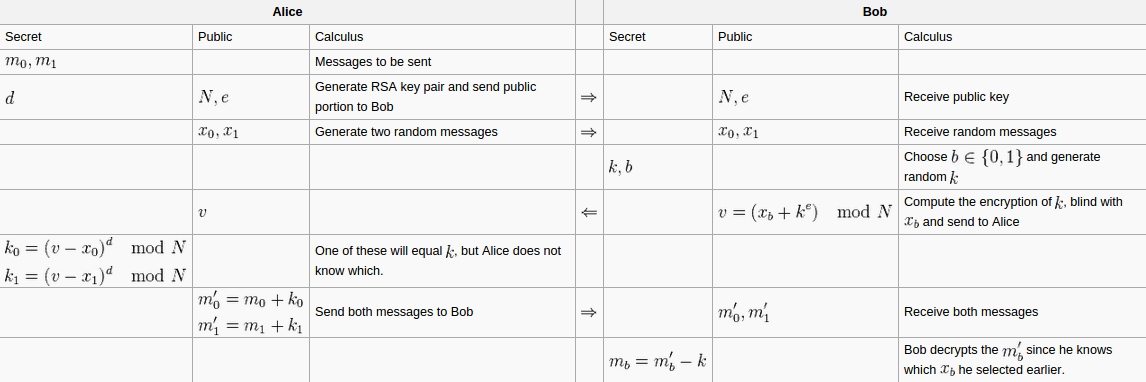
\includegraphics[scale=0.3]{images/ot_wiki}
    \caption{Semi-honest Naor-Pinkas oblivious transfer.}
\end{figure}

Researchers have also developed methods for performing k-out-of-n oblivious transfer, where the sender sends exactly $k$ messages out of a possible $n$.
The method described above is called $1-2$ oblivious transfer, and is the OT used in MPC protocols.

Since the first proposal of OT in \textbf{year}, several improvements have been developed.
Preprocessing.
OT extension.
Semi-honest/Malicious.

\subsection{Other}
\textbf{TODO}
Paper has topological circuit next to real circuit
change arbitrary function to arbitrary boolean function.

\section{Classic MPC}
MPC was first proposed by Andrew Yao in an oral presentation on secure function evaluation.
After Yao's presentation, two methods for performing MPC were developed.
One method was developed by Yao himself, and the other was developed by a group of researchers, Beaver, Micali and Widgerson.
The two methods are premised on a similar idea: encrypt a circuit by encrypting its gates, which has since been termed garbled circuit.
At this point, it is unclear which method is better, so researchers continue to study both methods.

This section will first give a new definition of a garbling scheme, first presented by BHR in 2012, and then give Yao's garbled circuit protocol, and finally GMW's garbled circuit protocol.

\subsection{Garbling Schemes}
Recall millionaires Alice and Bob who want to determine who has more wealth.
Alice and Bob start with a function $f$ (defined in \ref{function}) and their inputs, $x_a$ and $x_b$, which correspond to their amount of wealth.
In order to compute who has more money, the function $f$ needs to be transformed such that they can compute the function by sending messages between each other their inputs, $x_a$ and $x_b$, which correspond to their amount of wealth.
Informally, a garbling scheme transforms a specification of a function into a collection of algorithms which can in combination can compute the function.

\begin{definition}{Garbling Scheme}
    A garblering scheme is a $5$ tuple of algorithms $G = (\Gb, \En, \De, \Ev, \ev)$ where the algorithms are
    \begin{itemize}
        \item $\Gb(f, k) \rightarrow (F,e,d)$. 
        \item $\En(e,x) \rightarrow X$.
        \item $\Ev(F,X) \rightarrow Y$.
        \item $\De(d,Y) \rightarrow y$.
        \item $\ev(f, x) \rightarrow y$.
        where 
        \begin{itemize}
            \item $f$ is a function.
            \item $k \in \mathbb{N}$ is the security parameter.
            \item $x \in \{0,1\}^n$ is the initial input.
            \item $X$ is the garbled input
            \item $Y$ is the garbled output
            \item $y$ is the final output
            \item $F$ is a string that describes the operation of the $\Ev$ algorithm. 
            \item $e$ is a string describing the operation of the $\En$ algorithm. In particular, $e$ describes how to obscure the input $x$.
            \item $d$ is a string describing the operation of the $\De$ algorithm. In particular, $d$ describes how to unobscure the output $Y$.

        \end{itemize}
        \item A garbling scheme guarantees correctness if $\De(d, \Ev(F, \En(e,x))) = \ev(f,x)$.
    \end{itemize}
    A garbling schemes map the information:
\begin{equation}
    (f,k,x) \rightarrow^{\Gb} (F,e,d,x) \rightarrow^{\En} (F,d,X) \rightarrow^{\Ev} (d,Y) \rightarrow^{\De} y
\end{equation}
\end{definition}

To make the idea a garbling scheme more concrete, below is an example of how Alice and Bob would compute who is wealthier. 
The inputs to their computation are $f$, the function to be computed which is defined in equation \ref{eqn:less_than}, and their inputs $x_a$ and $x_b$.
\begin{enumerate}
    \item Alice has the function $f$ to be computed, her input $x_a$, and Bob has his input $x_b$.
    \item Alice hard-codes her inputs into the function, resulting in $\hat{f}$.
    \item Alice runs the probabilistic algorithm $\Gb(\hat{f}, k)$. She now has $(F,e,d)$.
    \item Alice encodes all possible inputs that Bob could, all possible sequences of $0$s and $1$s, into $X$ using $\En$.
    \item Alice sends $(F,X,d)$ to Bob.
    \item Bob runs $\Ev(F,X)$ to get $Y$. This computes the function, but the output, $Y$, is obscured.
    \item Bob runs $\De(d,Y)$ to get $y$. This unobscures the output $Y$. Bob now has $y \in \{0,1\}$.
        If $y = 0$, then Bob knows that Alice is wealthier. 
        If $y = 1$, then Bob knows that he is wealthier.
    \item Bob sends $y$ to Alice.
\end{enumerate}

The definition of a garbling scheme is a recently created definition, proposed for the first time ****, *** years after Yao's garbled circuit was proposed.
The benefits of thinking of a garbled scheme in terms of this definition are significant.
For one, it easier to map a theoretically garbling protocol into practice, i.e program it. 
The methods are already separated, whereas before the algorithm was generally one giant idea.
When the methods are separated, the programmer does not need to intimately understand the security guarantees and pitfalls of the method, as the sequence of events that need to happen is explicit in the construction.
A second reason that this definition of a garbling scheme is good is that it presents garbling as a larger cryptographic abstraction. 
Garbling schemes are simply methods for garbling a function and input, and this definition matches the intuition. 

\subsection{Projective Garbling Schemes}
Perhaps a helpful abstraction to have later.

\subsection{Security of Garbling Schemes}
This section will give the definition of security of a garbling scheme.

\subsection{MPC Security Definitions}
A number of definitions which formalize what it means for a multiparty computation have been formalized. 
Yao, in his 1982 paper on secure function evaluation, says a 2PC protocol is secure if it has the property:

\begin{blockquote}
If one participant behaves according the the protocol, the probability that the other participant successfully cheats is at most $\gamma$ for $\gamma \in \{0,1\}$.
\end{blockquote}

Since Yao's original definition, many other definitions for the security of 2PC protocols have been proposed.
Here we give Goldreich's definition of 2PC, which is given in his textbook \textit{Foundations of Cryptography Volume II}, and is reproduced in various papers, most notably Lindell and Pinkas 2009 survey paper on multiparty computation \cite{goldreich2, lindell2009}.

%As more complex protocols were developed, both for MPC, and in other areas of cryptography, property based definitions became difficult to work with.
%The main problem that it was unclear precisely what assumptions were being made about what each party could and couldn't do. 
%For example, in Yao's definition above, it's not clear that the parties' inputs are kept secret if both parties behave according to the protocol.
%At the least, the definition doesn't give any guarantee.
%For a while, cryptographers added in additional properties to definitions, but eventually it became clear that there was always the possibility that a certain property was being missed.

%This led to the creation to indistinguishability and simulation based definitions of security.
%The idea is that the adversary cannot tell what is going on, based on the information that they receive, so the best that the adversary can possible do is guess what is happening.
%For example, a definition of a secure encryption scheme could be:
%\textbf{Might give the definition of encryption in the section above. If we do, just reference that section. That might be preferable}

%\begin{blockquote}
%\begin{itemize}
%	\item Adversary picks two messages, $m_0$ and $m_1$. 
%	\item We pick a random bit $b \in \{0,1\}$. Encrypt $m_b$, and send the encrypted version to the adversary (i.e. send $c = \Enc(m_b)$).
%	\item Adversary outputs a bit $b'$ where $b' = 0$ if they believe the encrypted messages was $m_0$, and $b' = 1$ if they think the encrypted message was $m_1$. 
%	\item Finally, we consider the encryption scheme secure if
%	$$Pr[\text{Adversary outputs $b' = b$}] \approx_C \frac{1}{2}.$$
%\end{itemize}
%\end{blockquote}
%
%The cryptography research community now tends to prefer simulation based definitions. 
%The idea behind simulation based definitions is that we have ideal world, in which the protocol is run perfectly and securely, and then we have the real world protocol, the one that Alice and Bob run. 
%Then, for some adversary, we randomly choose either the real ideal or real world and run the MPC computation with the adversary in that world.
%The adversaries attempts to determine which world the protocol is being run in.
%Finally, the protocol is secure if the adversary can't do any better than guessing which world they are in.
%As a consequence, the real world is indistinguishable from the ideal world, hence cryptographers feel confident that the protocol is secure. 
%The idea being that if the adversary could learn more information in the real world, say information about other parties' inputs, then they would know that they are in the real world, hence the protocol is insecure. 
%
%The biggest problem with simulation based definitions is that it is difficult and labor intensive to prove with the definition.
%The property based definitions are the most straightforward to prove, and the most familiar to proofs used in mathematics.
%

\subsection{Goldreich and Lindell's Definition of Security for 2PC}
%The definition is designed for static, semi-honest adversaries. 

\begin{description}
\item [Setup:] \hfill
    \begin{itemize}
        \item Let $f = (f_1, f_2)$ be a probabilistic, polynomial time functionality. 

        \item Let $\Pi$ be a two party protocol for computing $f$. 

        \item Define $\viewrv_i^{\Pi}(n,x,y)$ (for $i \in \{1,2\}$) as the view of the $i$th party on input $(x,y)$ and security parameter $n$.
        $\viewrv_i^{\Pi}(n,x,y)$ equals the tuple $(1^n, x, r^i, m_1^i, \ldots, m_t^i)$, where $r^i$ is the contents of the $i$th party's internal random tape, and $m_j^i$ is the $j$th message that the $i$th party received.
    
        \item Define $output^{\Pi}_i(n,x,y)$ as the output of the $i$th party on input $(x,y)$ and security parameter $n$.
        Also denote
        $$ \outputrv^{\Pi}(n,x,y) = (\outputrv^{\Pi}_1(n,x,y), \outputrv^{\Pi}_2(n,x,y)).$$

    \item Note that $\viewrv^{\Pi}_i$ and $\outputrv^{\Pi}_i$ are random variables whose probabilities are taken over the random tapes of the two parties. Also note that for two party computation.
\end{itemize}
\item [Definition:]
We say that $\Pi$ securely computes $f$ in the presence of static semi-honest adversaries if there exists probabilistic polynomial time algorithms $S_1$ and $S_2$ such that for all $x,y \in \{0,1\}^*$, where $|x| = |y|$, the following are true:
\begin{equation} 
    \label{eqn:secdef1}
    \{(S_1(x, f_1(x,y), f(x,y)))\}_{x,y} \equiv^C \{(\viewrv^{\Pi}_1(x,y), \outputrv^{\Pi}(x,y)) \}_{x,y} 
\end{equation}
\begin{equation} 
    \label{eqn:secdef2}
    \{(S_2(x, f_2(x,y), f(x,y)))\}_{x,y} \equiv^C \{(\viewrv^{\Pi}_2(x,y), \outputrv^{\Pi}(x,y)) \}_{x,y} 
\end{equation}

\item[Intuition:]
    We think of $\viewrv^{\Pi}_i$ as all of the information that the $i$th has to operate with, such that any conclusion that the $i$th party can come to could be determined from $view^{\Pi}_i$.
    Moreover, $\outputrv^{\Pi}_i$ is simply a complicated way of writing the output of the $i$th party. 
    The value of $\outputrv^{\Pi}_i$ is computable from the tuple $\viewrv^{\Pi}_i$.

    Let's dig a little deeper into the meanings of equation \ref{eqn:secdef1} and \ref{eqn:secdef2}.
    They state that a probabilistic, polynomial time algorithm, denoted $S_1$ and $S_2$, which is given access \textit{only} to the party's input and output can compute the view of a party.
    For example, the definition requires that $S_1$ on input $(x, f(x,y))$ must be able to compute $\viewrv^{\Pi}_i(x,y)$, in particular the messages received by party 1, such that the generated view is indistinguishable from the actual view.
If there exists an algorithm that can perform the aforementioned task, then $\Pi$ does not adequately conceal information, so we should not consider $\Pi$ to be secure.

    Finally, the definition requires that $|x| = |y|$; however, this constraint can be overcome in practice by padding the shorter input.
\end{description}

The definition of security provided here only applies when adversaries are semi-honest (see \ref{semihonest section}).
Definitions of security in settings with malicious adversaries require substantially more complexity.
As a result, these definitions are often simulation based definitions.
They imagine an ideal world, where the function $f$ must be computed securely, and by a series of comparisons, show that the real world where $\Pi$ computes $f$ is essentially the same as the ideal world.
For an easy to understand security definition of 2PC with malicious adversaries, we refer to reader to \cite{lindell2009}.

\subsection{Yao's Garbled Circuit}
We now give an implementation of a generic 2PC protocol created by Yao \cite{yao}.
The protocol works for two parties; we will call party 1 Alice, denoted $A$, and party 2 Bob, denoted $B$, who have inputs $x$ and $y$ respectively.
Suppose $f$ is the function that Alice and Bob wish to compute.

Yao's protocol depends on first encoding the function $f$ as a circuit, as discussed in more detail in section \ref{sctn:circuits}, and then Alice and Bob together evaluate the circuit.

% (complexity - add to end) The number of round is constant.
% 1 OT per input wire of party B + enc/dec for each gate.

\begin{algorithm}
\caption{Garble Circuit}
\label{alg:garble}
\begin{algorithmic}
    \Require Circuit $f(x,\cdot)$ 
    \Ensure Populate garbled tables $f(x,\cdot).tables$.
\For{wire $w_i$ in $f(x,\cdot).wires$} 
    \State Generate two encryption keys, called garbled values, $W_i^0$ and $W_i^1$.
    \State Assign $(W_i^0, W_i^1)$ to $w_i$.
\EndFor \\

\For{gate $g$ in $f(x,\cdot).gates$}
    \State Let $w_i$ be $g$'s first input wire.
    \State Let $w_j$ be $g$'s second input wire.
    \State Let $w_k$ be $g$'s output wire.
    \For{$(u,v) \in \{(0,0), (0,1), (1,0), (1,1)\}$}
    \State $T_g[u,v] = \Enc_{W_i^u}( \Enc_{W_j^v} ( W_k^{g(u,v)}))$
    \EndFor
    \State $f(x,\cdot).tables[g] = T_g$.
\EndFor
\end{algorithmic}
\end{algorithm}

\begin{algorithm}
\caption{Evaluate Circuit}
\label{alg:evaluate}
\begin{algorithmic}

\Require $(input\_wires, tables, gates)$
\For{Input wire $w_i$ in $input\_wires$}
	\Comment retrieve garbled values of input wires
	\State Perform OT$(w_i, x_i)$ 
	\Comment retrieve $W^{x_i}_i$ from Alice
	\State Save the value to $w_i$.
\EndFor

\For{Gate $g$ in $gates$}
	\Comment compute the output of each gate.
	\State Let $w_i$ be $g$'s first input wire.
	\State Let $w_j$ be $g$'s second input wire.
	\State Let $w_k$ be $g$'s output wire.
	\State \textbf{Require} $w_i$ and $w_j$ have been assigned garbled values.
	\State \textbf{Require} $w_k$ has not been assigned a garbled value.
    	\For{$(u,v) \in \{(0,0), (0,1), (1,0), (1,1)\}$}
		\State $temp = \Dec_{w_j}(\Dec_{w_i}(tables[g][u,v]))$
		\If{$temp$ decrypted correctly}
			\State $w_k = temp$
		\EndIf
	\EndFor
\EndFor
\end{algorithmic}
\end{algorithm}

\subsubsection{Step 0: Setup}
Alice and Bob want to compute the function $f(x,y)$, where $x,y \in \{0,1\}^*$.
Alice is the garbler, and will create the circuit.
Bob is the evaluator, and will compute the circuit.
Alice first hardwires her inputs into the circuit, yielding a circuit that computes $f(x,\cdot)$.

\subsubsection{Step 1: Garbling the Circuit}
Alice garbles each gate, according to the algorithm outlined in Algorithm \ref{lag:garble}, which produces a table $T_g$ for each gate $g$.
The table enables the computation of $g$, if one is given either $W^0_i$ or $W^1_i$ and either $W^0_j$ or $W^1_j$ where wire $i$ and $j$ are the input wires to $g$.
Figure \ref{example} gives an example of a table for an AND gate. \textbf{TODO}

\subsubsection{Step 2: Bob's Input and Computing the Circuit}
Alice sends the garbled circuit to bob, which consists of the garbled tables, $f(x,\cdot).tables$, and the rules for connecting the gates together.
In order for Bob to compute the circuit, he needs the garbled values of all input wires.
Once he has the garbled values of the input wires, he can decrypt the first few gates, and acquire the decryption keys of the other gates until he has the keys to decrypt all of the gates in the circuit, yielding the output.
Bob can acquire the garbled values of the input wires from Alice using 1-out-of-2 oblivious transfer on each input wire (see section \ref{sctn:oblivious_transfer}).
If necessary, Bob sends the final output of the circuit to Alice. 
This is necessary only if $f_1(x,y) = f_2(x,y)$. 
Bob's protocol is outlined in more detail in Algorithm \ref{alg:evaluate}.

\subsubsection{Explanation of the security of Yao's protocol}
To do.

\subsubsection{Notes about complexity}
1 OT per (input?) wire.
How much encryption?
Not good enough for practice.

\subsection{GMW}
Where Yao's protocol is premised on encrypting gates individually, GMW's protocol for garbling circuits is premised on secret sharing, and performing operations on the shared secrets. 
Secret sharing, in its general idea, is class of methods for distributing a secret to a group of participants, where each participants is allocated a \textit{share} of the secret. 
The secret can only be reconstructed when a sufficient number of the participants combine their shares, but any pool of insufficient shares yields no information about the secret.

GMW begins by having Alice and Bob secret share their inputs, so each party now has a collection of \textit{shares}. 
Algorithm \ref{alg:gmw_setup} describes this process in more detail.
Then Alice and Bob perform a series of operations on their shares, which are dictated by the gates in the function they wish to compute.
As with Yao's protocol, a gate may either compute XOR, AND or NOT.
Each operation requires a different series of operations, which are described in Algorithm \ref{alg:gmw_gates}.
Finally, Alice and Bob publicize their shares to each other, at which point each party will have sufficient shares to compute the output of the function.

\begin{algorithm}[h!]
\caption{GMW Setup}
\label{alg:gmw_setup}
\begin{algorithmic}
% http://crypto.biu.ac.il/gmw-multi-party-protocol-and-oblivious-transfer-extension
    \State Alice does the following on input Circuit $f(x,\cdot)$ and $x = x_0x_1\ldots x_n$
    \For{wire $w_i$ in $f(x, \cdot).wires$}
        \State Assign $a^1_{w_i} \leftarrow \{0,1\}$
        \Comment a uniform random selection of $0$ or $1$.
        \State Assign $b^1_{w_i} = x_i \oplus a_{w_i}^1$
    \EndFor
    \State Bob does likewise on input Circuit $f(x,\cdot)$ and $y = y_0y_1\ldots y_n$
    \State Hence Alice has generated shares $\{a^1_w, b^1_w\}_w$ 
    \State and Bob has generated shares $\{a^2_w, b^2_w\}_w$
    \State Alice and Bob divide the shares such that Alice has all $a_w$ and Bob has all $b_w$.
\end{algorithmic}
\end{algorithm}

\begin{algorithm}
\caption{GMW Gate Evaluation}
\label{alg:gmw_gates}
\begin{algorithmic}
    \State \textbf{XOR Gate}
    \Comment $x_i \oplus y_i = (a_{w_i}^1 \oplus b_{w_i}^1) \oplus (a_{w_i}^2 \oplus a_{w_i}^2)$
    \State Alice evaluates $a_{w_i}^1 \oplus a_{w_i}^2$
    \State Bob evaluates $b_{w_i}^1 \oplus b_{w_i}^2$
    \\
    
    \State \textbf{AND Gate}
    \Comment $x_i \wedge y_i = (a_{w_i}^1 \oplus b_{w_i}^1) \wedge (a_{w_i}^2 \oplus a_{w_i}^2)$
    \State Alice samples $\sigma \leftarrow \{0,1\}$
    \Comment a uniform random selection of $0$ or $1$
    \State Alice constructs table $T$:
     \For{$(u,v) \in \{(0,0), (0,1), (1,0), (1,1)\}$}
     	\State $T[u,v] = (a^1_{w_i} \oplus u) \wedge (a^2_{w_i} \oplus v)$
	\State $s[u,v] = \sigma \oplus T[u,v]$.
     \EndFor    
     \State Do 1-4OT. Alice sends $(s[0,0], s[0,1], s[1,0], s[1,1])$ 
     \State Bob selects result based on $(u,v) = (b^1_{w_i}, b^2_{w_i})$.
    \\
    
    \State \textbf{NOT Gate}
    \Comment $w_i = (\neg a_{w_i}) \oplus (\neg b_{w_i})$
    \State $\triangleright$ Evaluate the negative of a particular wire $w_i$. 
    \State $w_i = a_{w_i} \oplus b_{w_i}$
    \State Let $a'_{w_i} = 1 \oplus a_{w_i}$
    \Comment i.e. $a'_{w_i} = \neg a_{w_i}$
    \State Let $b'_{w_i} = 1 \oplus b_{w_i}$
    \Comment i.e. $b'_{w_i} = \neg b_{w_i}$
\end{algorithmic}
\end{algorithm}

see mike rosulek first few slides for good images. 
illustrative about translating bits over to wire labels

\chapter{Improving MPC}
A number of improvements have been made to Yao's garbled circuit since its inception in 1986.
The first scheme for a garbled circuit, the one described in section \ref{garbled_circuit_scheme} has the following requirements: \textbf{include chart here}.
Let's look into how much work is required in classical garbled circuits.
\textbf{mention that we look gate-wise}
The first metric that we look at is the size of the garbled table.
\textbf{check this definition}:The garbled table, if you call recall from earlier, is the set of ciphertexts that is sent from the garbler to the evaluator, like in figure \ref{the fig thats a garbled table}.
Hence the size refers to the number of ciphertexts that an evaulator needs to compute a single gate.
The XOR column gives the size of the garbled table for an xor gate, and naturaly the AND columns gives the of the garbled table for an AND gate.
The cost associated with the size of a garbled table manifests in effecting the amount of bandwidth that needs to be transmitted between the garbler and evaluator.
In order to evaluate the gate, the evaluator needs the entire garbled table (\textbf{research idea: what if they don't? what if they can know when to request more information, to reduce the average amount of bandwidth? maybe this could be used to reduce calls to OT?)}, so reducing the size of the garbled table reduces bandwidth.
It turns out that bandwidth contributes a large hit to the total time required to perform mpc with garlbed circuits, and as a result, many of the improvements to garbled circuits have specifically targted reducing the size of the garbled table down from 4 ciphertexts.
\textbf{maybe mention lower bound?}

The second metric we use to analyze garbled circuits is eval cost.
Eval cost is the amount of computation that the evaluator must perform in order to process a single gate.
In the classical setting, the evaluator goes down the garbled table decrypting each ciphertext until one of the decrypts correctly. 
In the worst case, this requires 8 decryptions, because each wire is encrypted twice, once with the key from the first input wire and then again with the key from second input wire.
If a dual-key cipher (an encryption scheme that takes two keys, see section \ref{dkc section}), then the evaluator only needs to perform four decryptions in the worst case.
The metric that we consider is the garble cost of a gate. 
The garble cost of a gate is amount of computation that the garbler needs to perform.
The improvements to MPC have generally increased the garble cost; having the garbler do more work, can reduce the size of the garble table which reduces bandwidth, and can reduce the amount of computation the evaluator needs to perform \textbf{fact check this}.
Before the research of \cite{our_paper} and the research presented in this thesis, there were not substantial benefits to garbler preprocessing, that is having the garbler do work \textit{before} the actual computation time. 
We call this having the garbler do offline work, because they can do the work at their leisure, like at night when computers are less used.
Then the online work, when the actual comptuation is performed, is reduced.

As we walk through the improvements to Yao's garbled circuit, we are going to think about the improvements affect the three metrics described above.
It should also be noted before we begin that these are improvements to the the computation of a single gate.
Speedups on the gate level propagately widely through the computation of the entire garbled circuit.
For example, the computation of AES now requires approximatley $40,000$ gates, so reducing the number of ciphertexts being transmitted per gate by $1$, reduces the total amount of ciphertexts that need to be sent by $10,000$ - a substantial speedup indeed.

%\section{Overview of history}
%\begin{itemize}
%    \item working on specific function verse general functions
%    \item working on number of parties
%    \item making it work for sugarbeet auction
%    \item election potential?
%    \item auctions
%    \item ----- Mike talk -----
%    \item Things to think about:
%    \item hardness assumption (Mike does not focus on)
%    \item size: CTs/ per gate
%    \item computation required
%    \item Mike at 9:00 has cites to papers of big improvements
%    \item Focus is on improving each individual gate
%\end{itemize}

\section{Point and Permute}
Beaver, Micali and Rogaway contributed the first major improvement to Yao's garbled circuit in 1990.
A detail that I may or may not (\textbf{check this}) have left out in the description of Yao's garbled circuit is that the order of the garbled table needs to be permuted.
If the first key sent is always the key corresponding to the input wires's $0$ keys, then the evaluator can learn what the value of the input wires is - a violation of security.
The solution to this problem is easy: permute the order of the garbled table.
Now the evaulator trial decrypts each of the $4$ ciphertexts until there is a valid decryption .
\footnote{There exists encryption/decryption schemes that in addition to decrypting a ciphertext will also output a bit indicating if the decryption occurred correctly. Using schemes like this, the evaluator can decrypt all $4$ ciphertexts until one of them decrypts correctly, as indicated by the extra bit output by the decryption algorithm.}

The \textit{point and permute} technique speeds up the evaluator's computation of the garbled table by removing the need to trial decrypt the ciphertexts; instead, the garbler subtly communicates which single ciphertext to decrypt.
Using point and permute, the garbler randomly assigns a select bit $0$ or $1$ to each wire label in a wire \textbf{Is it clear what a wire label is, as opposed to a wire? Should be by now.}
The assignment of the select bit is independent of the truth value of the wire, so two things can happen. 
First, the garbler can permute the garbled table based on the select bits, and second, the select bits can be sent to the evaluator.
Upon receving the garbled table, the evaluator knows exactly which ciphertext to decrypt based on the select bits of the input wires.

Point and permute slightly increases the amoount of garbler-side computation to substantially decrease the amount of evaluator computation.
The garbler needs to sample $n+q$\footnote{Recall from \textbf{todo some previous section} that $n+q$ = number of wires.} additional random bits.
Without point and permute, the evaluator needs to decrypt $2.5$ ciphertexts on average, hence we estimate that there are roughly $1.5(n+q)$ fewer decryptions required.
The overall bandwidth is increased by $2$ bits per wire, from $256$ bits to $258$ bits: a small constant increase. \footnote{The value is constant in the sense that it is independent of the security parameter.}

\begin{table}[h]
    \centering
    \begin{tabular}{|c|c|}
    \hline
    Select Bit & Wire Label \\
    \hline
    0 & $A_0$ \\
    1 & $A_1$ \\
    1 & $B_0$ \\
    0 & $B_1$ \\
    \hline
    \end{tabular}
    \qquad
    \begin{tabular}{|c|c|}
    \hline
    Select Bits & Encryption \\
    \hline
    (0,0) & $\Enc_{A_0, B_1}(C_1)$ \\
    (0,1) & $\Enc_{A_0, B_0}(C_0)$ \\
    (1,0) & $\Enc_{A_1, B_1}(C_0)$ \\
    (1,1) & $\Enc_{A_1, B_0}(C_0)$ \\
    \hline
    \end{tabular}
    \qquad
    \begin{tabular}{|c|}
    \hline
    $C_0 \gets \{0,1\}^n$ \\
    $C_1 \gets \{0,1\}^n$ \\
    \hline
    \end{tabular}
    \caption{Garbled Gate for Point and Permute}
    \caption{Example garbled gate using point and permute. The gate being computed is given in figure \textbf{Make it 23:30 in mike's talk}}
\end{table}

\textbf{add chart if you want}

%\begin{itemize}
%    \item relative position of ciphertexts in table leaks information
%    \item so we have to permute the ciphertexts
%    \item when evaluating, trial decrypt all 4 until 1 works
%    \item beaver micali rogaway 90
%    \item randomly assign color (r,b) to each pair of wire label
%    \item Order the 4 cts canonically, by \emph{color} of keys: ((r,r),(r,b),(b,r),(b,b))
%    \item evaluate by decrypting ciphertexts indexed by your colors
%    \item Can use one-time-security encyption (e.g. OTP)
%    \item color independent of semantic value
%    \item show chart
%\end{itemize}

\section{Garbled Row Reduction 3}
Garbled Row Reduction 3 (GRR3) is technique proposed by \textbf{who} which decreases the number of ciphertexts that need be communicated between the garbler and evaluator.
To use GRR3, the garbler must also use the point and permute method.
Using Garbled Row Reduction, the garbler sets the ciphertext in the top row of the garbled table equal to a value that decrypts to $0^n$.
\footnote{In previous constructions the value for the ciphertext was chosen randomly.}
Upon evaluating the garbled gate, if the evaluator sees that the select bits of the input wires indicate to decrypt the first row, the evaluator simply assumes the ciphertext be of value $O^n$. 

\begin{table}[h]
    \centering
    \begin{tabular}{|c|c|}
    \hline
    Select Bit & Wire Label \\
    \hline
    0 & $A_0$ \\
    1 & $A_1$ \\
    1 & $B_0$ \\
    0 & $B_1$ \\
    \hline
    \end{tabular}
    \qquad
    \begin{tabular}{|c|c|}
    \hline
    Select Bits & Encryption \\
    \hline
    (0,1) & $\Enc_{A_0, B_0}(C_0)$ \\
    (1,0) & $\Enc_{A_1, B_1}(C_0)$ \\
    (1,1) & $\Enc_{A_1, B_0}(C_0)$ \\
    \hline
    \end{tabular}
    \qquad
    \begin{tabular}{|c|}
    \hline
    $C_0 \gets \{0,1\}^n$ \\
    $C_1 \gets \Enc_{A_0, B_1}^{-1}(0^n)$ \\
    \hline
    \end{tabular}
    \caption{Example garbled gate using point and permute and garbled row reduction 3. The gate being computed is given in figure \textbf{Make it 23:30 in mike's talk}}
\end{table}

Discuss security.

GRR3 does not have a significant effect on garbler side compuation.
The difference being that for constructing some wire lables, the garbler may need to compute $\Enc^{-1}$ instead of generating random bits. 
The evaluator needs to perform slightly less computation: in the event that the first row needs to be decrypted, the evaluator doesn't need to perform the decryption algorithm. 
This events occur with probabilty $\frac{1}{4}$, so we can extrapolate that the evaluator needs to perform $\frac{1}{4}$ fewer decryptions than wwould be necessary if only PP were being used.
GRR3 reduces the size of the garbled table from $4$ ciphertexts to $3$ ciphertexts, a $25\%$ reduction.

\section{Free XOR}
The Free XOR technique was developed by \textbf{who} in \textbf{when}.
The technique, as the name suggests, makes the computation of XOR gates essentially free.
Say the garbler is determining the lables for wire $A$.
The label associated with truth value $0$, $A_0$, is randomly sampled from $\{0,1\}^n$. 
Then the label assocated with the truth value is set such that $A_1 \gets A_0 \oplus \Delta$, where $\Delta$ is global, randomly sampled value from $\{0,1\}^n$.
If the garbler is garbling an XOR gate, then they set $C_0$ to $A \oplus B$, and like wire $A$, the garbler sets $C_1 = C_0 \oplus \Delta$.
With these wire labels, it turns out that the garbler doesn't need to send a garbled table: the evaluator can compute $C_0$ and $C_1$ by XORing the inputted wire labels.
The math for this operation is shown below:
\begin{align*}
    A \oplus B & = C \\
    (A \oplus \Delta) \oplus B & = (A \oplus B) \oplus \Delta = C \oplus \Delta \\
    A \oplus (B \oplus \Delta) & = (A \oplus B) \oplus \Delta = C \oplus \Delta \\
    (A \oplus \Delta) \oplus (B \oplus \Delta) & = (A \oplus B) \oplus (\Delta \oplus  \Delta) = C 
\end{align*}

\begin{table}[h]
    \centering
    \begin{tabular}{|c|c|}
    \hline
    Wire Label & Value\\
    \hline
    $A_0$ & $A$ \\
    $A_1$ & $A \oplus \Delta$ \\
    $B_0$ & $B$ \\
    $B_1$ & $B \oplus \Delta$ \\
    $C_0$ & $A \oplus B$ \\
    $C_1$ & $C_0 \oplus \Delta$ \\
    \hline
    \end{tabular}
    \qquad
    \begin{tabular}{|c|}
    \hline
    \hline
    \end{tabular}
    \caption{Example XOR garbled gate wires using PP, GRR3 and Free XOR.}
\end{table}

The Free XOR technique is also compatible with GRR3, but since XOR doesn't require a garbled table, GRR3 is only used on AND gates.

Using the Free XOR technique, the size of the garbled table is zero for all XOR gates and of size $3$ for AND gates.
This fact incentivizes the construction of circuits that optimize the number of XOR gates, minimize the number AND gates (while minimizing the size of the entire circuit of course).
One interesting implication of using the Free XOR technique is that an added assumption must be made to our encryption algorithm.
Since $\Delta$ is part of the key and part of the the payload\footnote{The payload is the value that is being encrypted} of the encryption algorithm, the encryption algorithm must be secure under the circularity assumption.
Fortunately, modern encryption uses AES-128, which is presumed to be secure under the circularity assumption.

%\begin{itemize}
%    \item post Fairplay
%    \item KolesnikovSchneider
%    \item $A,A \oplus \Delta$.
%    \item Note same delta every gate
%    \item Choose $C = A \oplus B$
%    \item XOR is then free: walk through that computatoin
%    \item Still works with GRR3
%    \item Because $\Delta$ is in the key and in the payload, requires circularity assumption
%    \item Incentivizes gates with as many xors as possible (has been done with AES -- why it's so fast)
%    \item Evaluator must konw what type of gate is being exectued: we have been assuming all along that the evaluator and garbler know the function.
%\end{itemize}

\section{Garbled Row Reduction 2}
Garbled row reduction 2 (GRR2) reduces the size of the garbled table for AND gates to $2$ ciphertexts, but it is not compatible with Free XOR, so XOR gates also require two ciphertexts.
The approach of GRR2 is quite different from GRR2. 
At a high level, it creates two third degree polynomials, one based on the input wires which should output $C_0$, and a second polynomial which should output $C_1$.
Since the polynomials are of three degrees, they are each uniquely generated by $3$ points. 
To construct the polynomials, the garbler uses $x,y,z$ for the first polynomail and $u,v,w$ for the second polynomial.
The garbler sends $x,y,u,v$ to the evaluator, who can interpolate the polynomial and plug in values $a,b,c$.

GRR2 is incompatible with Free XOR because the ciphertext values cannot be set to the xor of the inputer wires (e.g. $C \gets A \oplus B$), since the value of $C$ is always determined by the polynomial.

\textbf{Add to this, but no need to spend too much time on it since it's not used}

%\begin{itemize}
%    \item use unique deg-2 polynomial
%    \item use 2 second degree polynomials
%    \item then interpolate
%    \item can't do free xor.
%    \item because we have lost control of $C_0$ and $C_1$ (they are dependent on the polynomial)
%\end{itemize}

\section{FleXOR}
Before the creation of FlexXOR, MPC was at an awkward point where some circuits with a large amount of xors could be computed faster with Free XOR and circuits with fewer XORS could be computed faster with GRR2.
FleXOR serves as a method to reconcile GRR2 with Free XOR, solving the problem where the ciphertext values of AND gates are independent of $\Delta$.

FleXOR's construction is straightforward: use GRR2 on AND gates, and use Free XOR on XOR gates, correcting the delta value where necessary.
To correct the delta value, FleXOR adds in a unary gate that maps $A, A \oplus \Delta_1 \to A', A' \oplus \Delta_2$.

Suppose we have the following situation: we computing an XOR gate with input wires $A,B$ and output wire $C$.
Input wires $A$ and $B$ have each come from a different AND gate, so their labels are the result of the polynomial interpolation of GRR2.
To perform Free XOR, $A,B$ and $C$ need to be using the same delta value. 
The garbler adds an extra gate between $A$ and $B$ and the $XOR$ gate that adjusts their XOR value to the correct value.
The unary\footnote{Unary means has one input and one output.} gate maps $A,A \oplus \Delta_1 \to A', A' \oplus \Delta_2$, where $\Delta_2$ is the correct delta value for the XOR gate.

A garbled AND table costs $2$ ciphertexts, and a garbled XOR table costs $0,1$ or $2$ ciphertexts depending on how many ciphertexts need to be corrected.
This turns the creation of the circuit into a combinatorial optimization problem, where the offset of each wire needs to be determined to minimize the total cost of each XOR gate and be subject to the compatibility of GRR2 for AND gates.
Without doing too much (if any) optimization of the circuit, FleXOR usually requires $0$ or $1$ ciphertext in practice.

%\begin{itemize}
%    \item switch delta value: $A,A \oplus \Delta_1 \to A', A' \oplus \Delta_2$
%    \item cost a single ciphertext (after using GRR3 trick)
%    \item total cost 0,1,2 dependent on how many distinct deltas
%    \item make wire label outputs of AND gates based on polynomial interpolation (GRR2)
%    \item So we can do both free xor (which cost 0 CTs) and GRR2 (which cost 2 CTs per And gate + delta correction)
%    \item turns into combinatorial optimization problem: determine offset for each wire to minimize total cost of each xor gate + subject to compatibility of 2-CT row-reduction of AND gates.
%    \item in practice, seemed to usually require 0 or 1
%    \item still has circularity problem because based on free zor
%\end{itemize}

\section{Half Gates}
Half Gates is the most recent technique developed to improve Yao's garbled circuit.
The goal was to make AND gates cost 2 ciphertexts, and for Free XOR to always be free.
The methodology at high level is to make AND gates rely on Free XOR, so that AND gates result in values with the correct Free XOR delta.

%\begin{itemize}
%    \item Goal: make AND gates cost 2 and have free xor.
%    \item a high level way to think about it: make AND gates rely on free xor in some way
%    \item ``philosophical question'': What is the garbler knows in advance the truth value of one input wire?
%    \item e.g. AND gate and their input value is a false
%    \item turn into unary gate (either note gate or identity gate)
%    \item Use GRR3 trick to get one to disappear (GRR3 relies on point and permute, so that is happening too)
%    \item So use only 1 ciphertext.
%    \item What if evaluator knows the truth value on input wire?
%    \item someohow learn that have the false wire label
%    \item if AND gate, then know that will learn false
%    \item similar thing with above with not and identity gate
%    \item cost 1 CT.
%    \item No need for point and permute here: because evaluator does different things based on having true or false wire label (and the assumption is that they know)
%    \item Real thing:
%    \item two halves make a whole!
%    \item compatible with free xor
%    \item AND gate requires two CTs
%    \item don't need to make $r$, we have a convenient $r$ floating around
%    \item r = color bit of FALSE wire label A
%    \item $a \oplus r$ = color bit of wire label evaluator gets ($A$ or $A \oplus \Delta)$
%    \item no polynomial interpolation at all -- i.e. not based on GRR2
%    \item every garbling scheme is a combo of
%    \item 1. symmetric primitive (PRF/hash function) (can be modeled as random oracle
%    \item 2. $GF((2^{\lambda}$-linear operators (XOR, polynomial interpolation)
%    \item Garbling a single AND gate requires 2 CTS ($2 \lambda$ bits) if garbling scheme is ``linear'' in this sense.
%    \item hence half-gates is size optimal: use ``known techniques'' and work gate-by-gate basis 
%\end{itemize}

\begin{table}[h]
  \centering
  \renewcommand{\arraystretch}{1.2}
\begin{adjustbox}{width=1\textwidth}
  \begin{tabular}{|p{5cm}||c|c||c|c||c|c||c|}
    \hline
    \multirow{2}{5cm}{\centering \textbf{Mode Transition Times Duration (Typical)}} & 
    \multicolumn{2}{c|}{\textbf{Size (x$\lambda$)}} & 
    \multicolumn{2}{c|}{\textbf{Eval Cost}} & 
    \multicolumn{2}{c|}{\textbf{Garble Cost}} &
    \multirow{2}{3cm}{\centering \textbf{Assumption}} \\
    \cline{2-7}
    & \textbf{XOR} & \textbf{AND} & \textbf{XOR} & \textbf{AND}  & \textbf{XOR} & \textbf{AND} & \\
    \hline
    Classical & 1365 & 1260 & 1024 & $\mu$ s & a & b & a\\ \hline
    Point and Permute & TBD & TBD & TBD & $\mu$ s & a & b & a\\ \hline
    GRR3 & TBD & TBD & TBD & $\mu$ s  & a & b& a\\ \hline
    Free XOR & TBD & TBD & TBD & $\mu$ & a & bs& a  \\ \hline
    GRR2 XOR & TBD & TBD & TBD & $\mu$ & a & bs  & a\\ \hline
    FleXOR& TBD & TBD & TBD & $\mu$ & a & bs & a \\ \hline
    Half Gates & TBD & TBD & TBD & $\mu$ & a & bs & a \\ \hline
  \end{tabular}
  \end{adjustbox}
  \caption{Summary of Garbled Circuit Improvements. GRR3 stands for garbled row reduction 3 and GRR2 stands for garbled row reduction 2}
\end{table}


\chapter{Template tips}
This is the first page of the first chapter. You may delete the contents of this chapter so you can add your own text; it's just here to show you some examples. 
	
\subsection{Footnotes and Endnotes}
	You might want to footnote something.\footnote{footnote text} Be sure to leave no spaces between the word immediately preceding the footnote command and the command itself. The footnote will be in a smaller font and placed appropriately. Endnotes work in much the same way. More information can be found about both on the CUS site.
	
\section{Bibliographies}
	Of course you will need to cite things, and you will probably accumulate an armful of sources. This is why BibTeX was created. For more information about BibTeX and bibliographies, see our CUS site (\url{web.reed.edu/cis/help/latex/index.html})\footnote{\cite{reedweb:2007}}. There are three pages on this topic: {\it bibtex} (which talks about using BibTeX, at \url{/latex/bibtex.html}), {\it bibtexstyles} (about how to find and use the bibliography style that best suits your needs, at \url{/latex/bibtexstyles.html}) and {\it bibman} (which covers how to make and maintain a bibliography by hand, without BibTeX, at at \url{/latex/bibman.html}). The last page will not be useful unless you have only a few sources. There used to be APA stuff here, but we don't need it since I've fixed this with my apa-good natbib style file.
	
\subsection{Tips for Bibliographies}
\begin{enumerate}
\item Like with thesis formatting, the sooner you start compiling your bibliography for something as large as thesis, the better. Typing in source after source is mind-numbing enough; do you really want to do it for hours on end in late April? Think of it as procrastination.
\item The cite key (a citation's label) needs to be unique from the other entries.
\item When you have more than one author or editor, you need to separate each author's name by the word ``and'' e.g.\\ \verb+Author = {Noble, Sam and Youngberg, Jessica},+.
\item Bibliographies made using BibTeX (whether manually or using a manager) accept LaTeX markup, so you can italicize and add symbols as necessary.
\item To force capitalization in an article title or where all lowercase is generally used, bracket the capital letter in curly braces.
\item You can add a Reed Thesis citation\footnote{\cite{noble:2002}} option. The best way to do this is to use the phdthesis type of citation, and use the optional ``type'' field to enter ``Reed thesis'' or ``Undergraduate thesis''. Here's a test of Chicago, showing the second cite in a row\footnote{\cite{noble:2002}} being different. Also the second time not in a row\footnote{\cite{reedweb:2007}} should be different. Of course in other styles they'll all look the same.
\end{enumerate}
\section{Anything else?}
If you'd like to see examples of other things in this template, please contact CUS (email cus@reed.edu) with your suggestions. We love to see people using \LaTeX\ for their theses, and are happy to help.

\chapter*{Conclusion}
         \addcontentsline{toc}{chapter}{Conclusion}
	\chaptermark{Conclusion}
	\markboth{Conclusion}{Conclusion}
	\setcounter{chapter}{4}
	\setcounter{section}{0}
	
Here's a conclusion, demonstrating the use of all that manual incrementing and table of contents adding that has to happen if you use the starred form of the chapter command. The deal is, the chapter command in \LaTeX\ does a lot of things: it increments the chapter counter, it resets the section counter to zero, it puts the name of the chapter into the table of contents and the running headers, and probably some other stuff. 

So, if you remove all that stuff because you don't like it to say ``Chapter 4: Conclusion'', then you have to manually add all the things \LaTeX\ would normally do for you. Maybe someday we'll write a new chapter macro that doesn't add ``Chapter X'' to the beginning of every chapter title.

\section{More info}
And here's some other random info: the first paragraph after a chapter title or section head \emph{shouldn't be} indented, because indents are to tell the reader that you're starting a new paragraph. Since that's obvious after a chapter or section title, proper typesetting doesn't add an indent there. 


%If you feel it necessary to include an appendix, it goes here.
    \appendix
      \chapter{The First Appendix}
      \chapter{The Second Appendix, for Fun}


%This is where endnotes are supposed to go, if you have them.
%I have no idea how endnotes work with LaTeX.

  \backmatter % backmatter makes the index and bibliography appear properly in the t.o.c...

% if you're using bibtex, the next line forces every entry in the bibtex file to be included
% in your bibliography, regardless of whether or not you've cited it in the thesis.
    \nocite{*}

% Rename my bibliography to be called "Works Cited" and not "References" or ``Bibliography''
% \renewcommand{\bibname}{Works Cited}

%    \bibliographystyle{bsts/mla-good} % there are a variety of styles available; 
%  \bibliographystyle{plainnat}
% replace ``plainnat'' with the style of choice. You can refer to files in the bsts or APA 
% subfolder, e.g. 
 \bibliographystyle{APA/apa-good}  % or
 \bibliography{thesis}
 % Comment the above two lines and uncomment the next line to use biblatex-chicago.
 %\printbibliography[heading=bibintoc]

% Finally, an index would go here... but it is also optional.
\end{document}
